\documentclass[c]{beamer}
\usepackage[latin1]{inputenc} 
\usepackage[T1]{fontenc}
\usepackage[francais]{babel}
\usepackage{verbatim}


\author{Nicolas Blanchard, Axel Davy et Marc Heinrich}
\institute{Ecole Normale Supérieure}
\date{Mardi 22 janvier 2013}

\begin{document}

\begin{frame}
  \maketitle
\end{frame}

\section{Summary}
\begin{frame}
  \tableofcontents
\end{frame}

\section{Processor details}

\subsection{Inner working}
\begin{frame}
  \frametitle{Fonctionnement}
  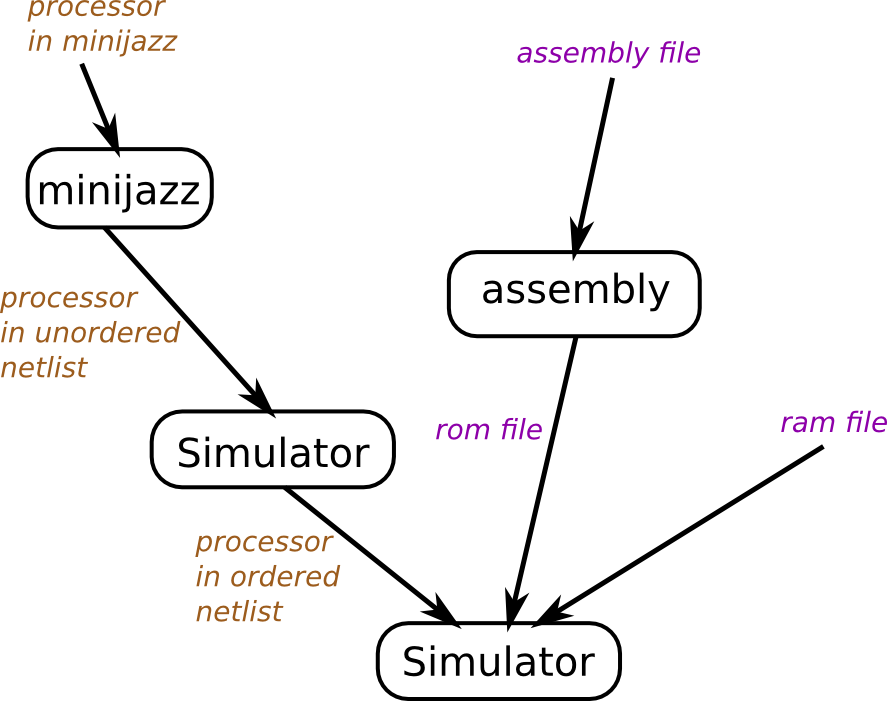
\includegraphics[scale=0.4]{schema_fonctionnement.png}
\end{frame}

\subsection{Le Simulateur}

\begin{frame}
\begin{itemize}
\item associate to each variable appearing in the netlists equations a cell in a table containing its value
\item two other tables are used to store the content of the RAM and the ROM (initialized with the files given in argument)
\item the netlist equations are applied in a sepecific order.
\item outputs values, or eventually some of the cells in the RAM table are printed into the standard output.
\item the process goes on until it reaches the number of steps asked by the users.
\end{itemize}
\end{frame}

\begin{frame}
Wich order? 
 % maybe some explanations here, or something else

\end{frame}

\subsection{Assembleur - fichier rom}

\begin{frame}
The Assebly takes in input a file written in an assembly language and outputs an array of '0's and '1's corresponding to the inital values of the ROM.

%We can put some of the architecture here
%maybe important instructions supported by our processor
%labels inplemented
%
\end{frame}

\begin{frame}

\end{frame}

\begin{frame}
\frametitle{Programme de l'horloge}
%maybe a picture of the assembly file (and a part of the rom file?)
\end{frame}

\subsection{Fichier ram}

\begin{frame}

\end{frame}

\subsection{Processor architecture}

\begin{frame}
\frametitle{The processor}
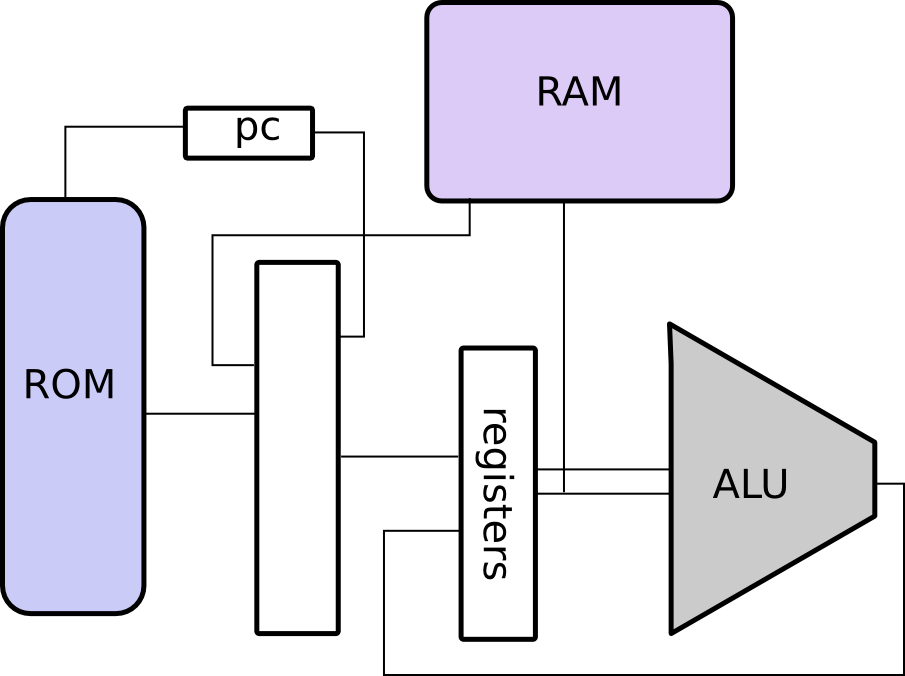
\includegraphics[scale=0.4]{schema_proc.png}

\end{frame}

\begin{frame}
\frametitle{Advantages}
\end{frame}

\section{Un travail d'équipe}

\begin{frame}
\frametitle{organisation du travail}
%github, mails, etc...
%how the work was split (for the simulator) 
\end{frame}

\section{Démonstration}

\begin{frame}

\end{frame}


\end{document}